\section{Vetor campo elétrico. Cargas puntiformes}

\setmyunit{1.5cm}

\frame{
	\frametitle{Vetor campo elétrico}
	\begin{block}{Introdução}
		Imagine um ponto $P$ situado em uma região onde há um campo elétrico. Inicialmente, nesse ponto, \textbf{não existe nenhuma carga elétrica}.
	\end{block}

	\vspace{0.3cm}
	
	\centering
	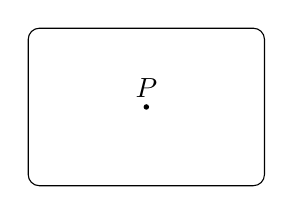
\begin{tikzpicture}
		\draw[rounded corners] (0,0) rectangle coordinate[] (p) (3,2) ;
		\fill (p) circle (1pt);
		\node[above] at (p) {$ P $};
	\end{tikzpicture}
	
%	\centerline{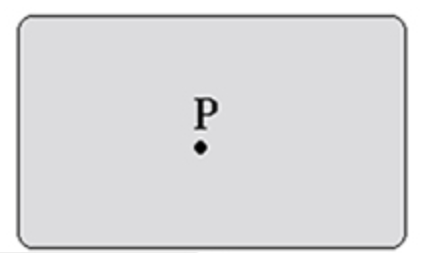
\includegraphics[width=0.4\linewidth]{Figuras/Ch07/vetor1.PNG}}
}

\frame{
	\frametitle{Vetor campo elétrico}
	\begin{block}{Introdução}
		Suponha agora colocar uma partícula eletrizada com carga $q_1$, carga de prova, exatamente no ponto $P$. Sobre a partícula, passa a atuar uma força de intensidade elétrica $\vec{F_1}$
	\end{block}

	\vspace{0.3cm}
	
	\centering
	\begin{tikzpicture}
	\draw[rounded corners] (0,0) rectangle coordinate[] (p) (3,2) ;
	
	\draw[-Latex,red] (p) -- node[above] {$ \vec{F_1} $} +(1,0);
	
	\fill (p) circle (1pt);
	\node[above] at (p) {$ P $};
	\node[below] at (p) {$ q_1 $};
	
	\end{tikzpicture}
%	\centerline{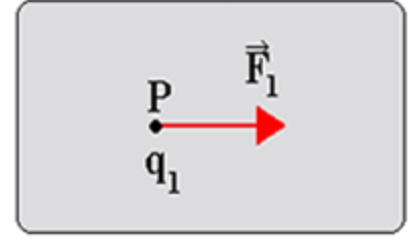
\includegraphics[width=0.4\linewidth]{Figuras/Ch07/vetor2.PNG}}
}

\frame{
	\frametitle{Vetor campo elétrico}
	\begin{block}{Introdução}
		Caso a carga de prova seja trocada por outra $q_2$, surge uma nova força elétrica na carga de prova, ou seja, surge a força elétrica $\vec{F_2}$.
	\end{block}

	\vspace{0.3cm}
	
	\centering
	\begin{tikzpicture}
	\draw[rounded corners] (0,0) rectangle coordinate[] (p) (3,2) ;
	
	\draw[-Latex,red] (p) -- node[above] {$ \vec{F_2} $} +(-1,0);
	
	\fill (p) circle (1pt);
	\node[above] at (p) {$ P $};
	\node[below] at (p) {$ q_2 $};
	
	\end{tikzpicture}
%	\centerline{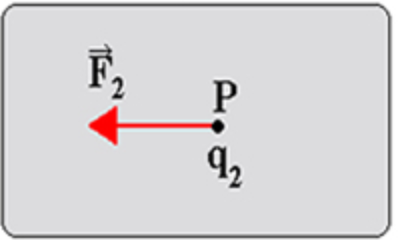
\includegraphics[width=0.4\linewidth]{Figuras/Ch07/vetor3.PNG}}
}

\frame{
	\frametitle{Vetor campo elétrico}
	\begin{block}{O que se percebe?}
		As forças possuem a mesma direção, porém a força que age sobre a carga positiva tem um dado sentido e a força que atua sobre a carga negativa tem sentido contrário.
	\end{block}

	\vspace{0.3cm}

	\begin{minipage}{0.49\linewidth}
%		\setmyunit{1.5cm}
		\centering
		\begin{tikzpicture}
		\draw[rounded corners] (0,0) rectangle coordinate[] (p) (3,2) ;
		
		\draw[-Latex,red] (p) -- node[above] {$ \vec{F_1} $} +(1,0);
		
		\fill (p) circle (1pt);
		\node[above] at (p) {$ P $};
		\node[below] at (p) {$ q_1 $};
		
		\end{tikzpicture}
	\end{minipage}
	\hfill
	\begin{minipage}{0.49\linewidth}
%		\vspace{0.3cm}
		\centering
		\begin{tikzpicture}
		\draw[rounded corners] (0,0) rectangle coordinate[] (p) (3,2) ;
		
		\draw[-Latex,red] (p) -- node[above] {$ \vec{F_2} $} +(-1,0);
		
		\fill (p) circle (1pt);
		\node[above] at (p) {$ P $};
		\node[below] at (p) {$ q_2 $};
		
		\end{tikzpicture}
	\end{minipage}
	
%	\centerline{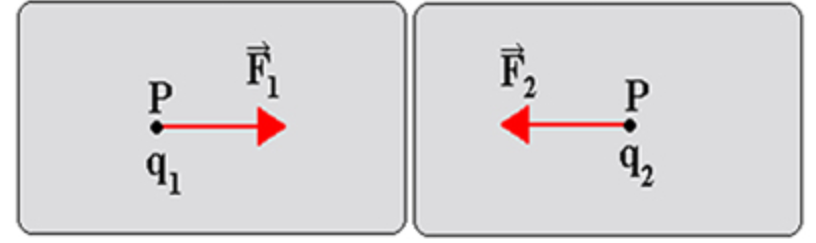
\includegraphics[width=0.8\linewidth]{Figuras/Ch07/vetor4.PNG}}
}

\frame{
	\frametitle{Vetor campo elétrico}
	\begin{block}{Definição}
		O campo elétrico é definido como um \textbf{vetor} com \textbf{mesma direção} do vetor da força de interação entre a carga geradora $Q$ e a carga de prova $q$ e com \textbf{mesmo sentido} se $q>0$ e \textbf{sentido oposto} se $q<0$.
	\end{block}
}

\frame{
	\frametitle{Vetor campo elétrico}
	\begin{block}{Vetor característico}
		Tanto experimentalmente como teoricamente, fazendo-se a razão entre a força atuante em cada partícula e o valor algébrico da carga onde ela atua, \textbf{o resultado é sempre o mesmo}, ou seja,
		$$\dfrac{\vec{F_1}}{q_1} = \dfrac{\vec{F_2}}{q_2} = ... = \dfrac{\vec{F_n}}{q_n} \ \ \text{(constante)}$$ \\
		\begin{itemize}
			\item Se a razão permanece constante, isso significa que ela não depende dos valores de $\vec{F}$ ou de $q$, constituindo um vetor característico daquele ponto do campo elétrico.
		\end{itemize}
	\end{block}
}

\frame{
	\frametitle{Vetor campo elétrico}
	\begin{block}{Formulação matemática}
		Da definição de campo elétrico $\vec{E}$ podemos escrever
		$$\vec{F} = q \ \vec{E}$$ \\
		Portanto, o vetor $\vec{F}$ é expresso pelo produto de um número real $q$ por um vetor $\vec{E}$. Evidentemente, o vetor $\vec{E}$ e o vetor $\vec{F}$ terão sempre a mesma direção, desde que não sejam nulos.
		\begin{enumerate}
			\item $q > 0$: $\vec{E}$ tem o mesmo sentido de $\vec{F}$.
			\item $q < 0$: $\vec{E}$ tem o sentido oposto de $\vec{F}$.
		\end{enumerate}
	\end{block}
}

\frame{
	\frametitle{Vetor campo elétrico}
	\begin{block}{Em resumo}
		O vetor campo elétrico apresenta as seguintes características: \\
		\begin{itemize}
			\item \textbf{Módulo}: o módulo do campo elétrico em um ponto $P$ é dado por $\vec{E} = \vec{F}/q$
			\item \textbf{Direção}: é a mesma da força elétrica.
			\item \textbf{Sentido}: é o mesmo da força elétrica se $q > 0$ e sentido contrário se $q < 0$.
		\end{itemize}
	\end{block}
}

\frame{
	\frametitle{Vetor campo elétrico}
	
	\setmyunit{0.5cm}
	
	\begin{minipage}{0.49\linewidth}
		\centering
		
		\begin{tikzpicture}
			\draw (0,0) circle (1) node {\LARGE $ + $};
			\draw (-3,-3) circle (0.5) node {$ + $};
			
			\draw[dashed] (0,0) +(45:-1) -- ($ (-3,-3)+(45:0.5) $);
			
			\draw[-Latex,green] ($ (-3,-3)+(45:-0.5) $) -- +(45:-2) node[midway,above left=0.1] {$ \vec{F} $};
			
			\draw[-Latex,red] ($ (-3,-3)+(45:-0.5) $) -- +(45:-1) node[midway,below right] {$ \vec{E} $};
		\end{tikzpicture}
	\end{minipage}
	\hfill
	\begin{minipage}{0.49\linewidth}
		\centering
		
		\begin{tikzpicture}
		\draw (0,0) circle (1) node {\LARGE $ - $};
		\draw (-3,-3) circle (0.5) node {$ + $};
		
		\draw[dashed] (0,0) +(45:-1) -- ($ (-3,-3)+(45:0.5) $);
		
		\draw[-Latex,green] ($ (-3,-3)+(45:0.5) $) -- +(45:2) node[midway,above left=0.05] {$ \vec{F} $};
		
		\draw[-Latex,red] ($ (-3,-3)+(45:0.5) $) -- +(45:1) node[midway,below right] {$ \vec{E} $};
		\end{tikzpicture}
	\end{minipage}

	\begin{minipage}{0.49\linewidth}
		\centering
		
		\begin{tikzpicture}
		\draw (0,0) circle (1) node {\LARGE $ + $};
		\draw (-3,-3) circle (0.5) node {$ - $};
		
		\draw[dashed] (0,0) +(45:-1) -- ($ (-3,-3)+(45:0.5) $);
		
		\draw[-Latex,green] ($ (-3,-3)+(45:0.5) $) -- +(45:2) node[midway,above left=0.05] {$ \vec{F} $};
		
		\draw[-Latex,red] ($ (-3,-3)+(45:-0.5) $) -- +(45:-1) node[midway,below right] {$ \vec{E} $};
		\end{tikzpicture}
	\end{minipage}
	\hfill
	\begin{minipage}{0.49\linewidth}
		\centering
		
		\begin{tikzpicture}
		\draw (0,0) circle (1) node {\LARGE $ - $};
		\draw (-3,-3) circle (0.5) node {$ - $};
		
		\draw[dashed] (0,0) +(45:-1) -- ($ (-3,-3)+(45:0.5) $);
		
		\draw[-Latex,green] ($ (-3,-3)+(45:-0.5) $) -- +(45:-2) node[midway,above left=0.1] {$ \vec{F} $};
		
		\draw[-Latex,red] ($ (-3,-3)+(45:0.5) $) -- +(45:1) node[midway,below right] {$ \vec{E} $};
		\end{tikzpicture}
	\end{minipage}
%	\centerline{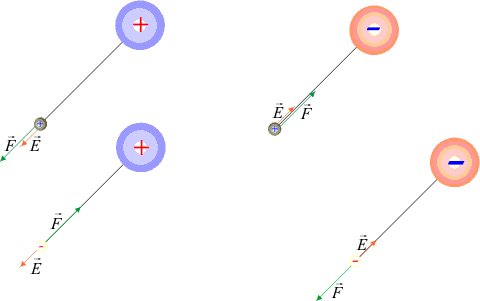
\includegraphics[width=1\linewidth]{Figuras/Ch07/campoeforca.png}}
}

\frame{
	\frametitle{Vetor campo elétrico}
	\begin{block}{Importante}
		Quando a carga geradora do campo tem sinal positivo ($Q>0$), o vetor campo elétrico tem \textbf{sentido de afastamento} das cargas e quando tem sinal negativo ($Q<0$), tem \textbf{sentido de aproximação}, sendo que isto não varia com a mudança do sinal das cargas de provas.
	\end{block}
}

\frame{
	\frametitle{Campo elétrico de várias cargas pontuais fixas}
	\begin{block}{Motivação}
		O que fazer quando temos várias cargas gerando o campo elétrico? A primeira coisa que precisamos saber é que \textbf{cada carga elétrica está associada ao seu campo elétrico}, ou seja, sabemos que cada carga elétrica “cria” seu campo elétrico.
	\end{block}
	
%	\vspace{0.3cm}
	
	\centering
	\begin{tikzpicture}
		\draw[dashed] (0,0) -- (60:1.5) (0,0) -- (120:1.5) (0,0) -- (1.5,0);
		
		\filldraw[fill=white] (60:1.5) circle (8pt) node["$ Q_2 $" above] {$ - $} (120:1.5) circle (8pt) node["$ Q_1 $" above] {$ + $} (1.5,0) circle (8pt) node["$ Q_3 $" above] {$ - $};
		
		\draw[-Latex] (0,0) -- node[above left] {$ \vec{E_2} $} (60:1);
		\draw[-Latex] (0,0) -- node[right] {$ \vec{E_1} $} (-60:1);
		\draw[-Latex] (0,0) -- node[above] {$ \vec{E_3} $} (1,0);
		
		\fill (0,0) circle (3pt);
	\end{tikzpicture}
	
%	\centerline{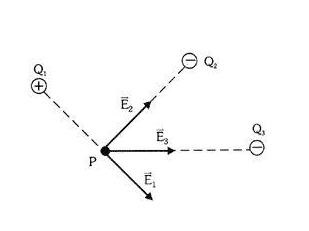
\includegraphics[width=0.6\linewidth]{Figuras/Ch07/varias1.jpg}}
}

\frame{
	\frametitle{Campo elétrico de várias cargas pontuais fixas}
	\begin{block}{Definição}
		Quando o campo elétrico é criado por várias cargas puntiformes fixas, $Q_1$, $Q_2$,..., $Q_N$ podemos determinar o campo elétrico originado por essas cargas num ponto $P$ qualquer do espaço. \\
		\vspace{0.5cm}
		Se $Q_1$ estivesse sozinha, originaria em $P$ o vetor campo $\vec{E_1}$; bem como $Q_2$ sozinha, originaria em $P$ um vetor campo $\vec{E_2}$ e assim por diante, até $Q_N$ que, sozinha, geraria o vetor campo $\vec{E_N}$. \\
		\vspace{0.5cm}
		\begin{itemize}
			\item O \textbf{vetor campo elétrico resultante} no ponto $P$, em razão de várias cargas é a soma vetorial dos campos $\vec{E_1}$, $\vec{E_2}$, $\vec{E_N}$, onde cada vetor parcial é determinado como se a carga respectiva estivesse sozinha. Ou seja,
		\end{itemize}
		$$\vec{E} = \vec{E_1} + \vec{E_2} + ... + \vec{E_N}$$
	\end{block}
}

\frame{
	\frametitle{Campo elétrico de várias cargas pontuais fixas}
	\begin{block}{Uma possibilidade...}
		Como as duas cargas geradoras do campo têm sinal positivo, cada uma delas gera um campo divergente (de afastamento), logo o vetor resultante terá módulo igual à subtração entre os valores dos vetores e direção e sentido do maior valor absoluto. \\
		$$\vec{E_R} = \vec{E_A} + \vec{E_B}$$
	\end{block}

	\vspace{0.3cm}
	
	\centering
	\begin{tikzpicture}
		\draw[dashed] (-2,0) -- (2,0);
		
		\draw[-Latex] (0,0) -- node[above] {$ \vec{E_A} $} (1.5,0);
		\draw[-Latex] (0,0) -- node[above] {$ \vec{E_B} $} (-1,0);
		
		\fill (0,0) circle (3pt) node[below=2pt] {$ P $};
		
		\filldraw[fill=white] (-2,0) circle (8pt) node[below=8pt] {$ A $} node["$ Q_A $" above] {$ + $} (2,0) circle (8pt) node[below=8pt] {$ B $} node["$ Q_B $" above] {$ + $};
	\end{tikzpicture}
%	\centerline{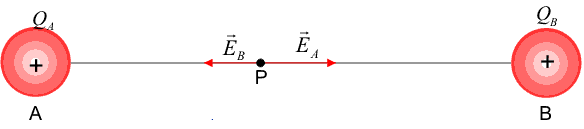
\includegraphics[width=0.6\linewidth]{Figuras/Ch07/varias2.png}}
}

\frame{
	\frametitle{Campo elétrico de várias cargas pontuais fixas}
	\begin{block}{Outra possibilidade...}
		Assim como no exemplo anterior, ambos os campos elétricos gerados são divergentes, mas como existe um ângulo formado entre eles, esta soma vetorial é calculada através de regra do paralelogramo, ou seja, traçando-se o vetor soma dos dois vetores, tendo assim o módulo direção e sentido do vetor campo elétrico resultante. \\
		$$\vec{E_R} = \vec{E_A} + \vec{E_B}$$
	\end{block}

%	\vspace{0.3cm}
	
	\setmyunit{1cm}
	
	\centering
	\begin{tikzpicture}[]
	\draw[dashed] (-2,0) -- (1.5,0) coordinate (A) (-60:2) -- (120:1.5);
	\draw[dashed,red] (120:1) -- +(1.5,0) (1,0) -- +(120:1.5);
	
	\draw[-Latex] (0,0) coordinate (O) -- node[below] {$ \vec{E_A} $} (1,0);
	\draw[-Latex] (0,0) -- node[left] {$ \vec{E_B} $} (120:1) coordinate (B);
	
	\draw[-Latex,red] (0,0) -- (60:1) node[above,xshift=5pt] {$ \vec{E_R} $};
	
	\fill (0,0) circle (3pt) node[below left=2pt] {$ P $};
	
	\filldraw[fill=white] (-2,0) circle (8pt) node[below=8pt] {$ A $} node["$ Q_A $" above] {$ + $} (-60:2) circle (8pt) node[right=8pt] {$ B $} node["$ Q_B $" above] {$ + $};
	
	\pic[ang,gray,->,"$ \alpha $" {xshift=3pt,yshift=-3pt}] {angle=A--O--B};
	\end{tikzpicture}
%	\centerline{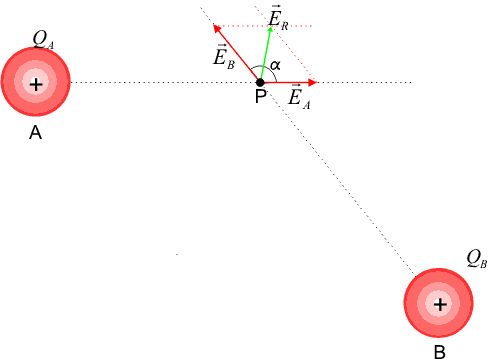
\includegraphics[width=0.4\linewidth]{Figuras/Ch07/varias3.png}}
}

\frame{
	\frametitle{Campo elétrico de várias cargas pontuais fixas}
	\begin{block}{Mais uma possibilidade...}
		Como ambas as cargas que geram o campo tem sinais negativos, cada componente do vetor campo resultante é convergente, ou seja, tem sentido de aproximação. O módulo, a direção e o sentido deste vetor são calculados pela regra do paralelogramo. \\
		$$\vec{E_R} = \vec{E_A} + \vec{E_B}$$
	\end{block}

	\setmyunit{1cm}
	
	\centering
	\begin{tikzpicture}[]
	\draw[dashed] (-2,0) -- (0.5,0) (-120:2) -- (60:0.5);
	
	\draw[-Latex] (0,0) coordinate (O) -- node[above] {$ \vec{E_A} $} (-1,0) coordinate (A);
	\draw[-Latex] (0,0) -- node[right] {$ \vec{E_B} $} (-120:1) coordinate (B);
	
	\draw (A) +(-120:1) coordinate (Ad);
	
	\draw[-Latex,red] (0,0) -- (Ad) node[below left,xshift=-5pt] {$ \vec{E_R} $};
	
	\draw[dashed,red] (A) -- (Ad) -- +(-0.5,0) (B) -- (Ad) -- +(-120:0.5);
	
	\fill (0,0) circle (3pt) node[above right=2pt,xshift=3pt] {$ P $};
	
	\filldraw[fill=white] (-2,0) circle (8pt) node[below=8pt] {$ A $} node["$ Q_A $" above] {$ - $} (-120:2) circle (8pt) node[below=8pt] {$ B $} node["$ Q_B $" above] {$ - $};
	
	\pic[ang,gray,->,"$ \alpha $" {xshift=3pt,yshift=-3pt}] {angle=A--O--B};
	\end{tikzpicture}
%	\centerline{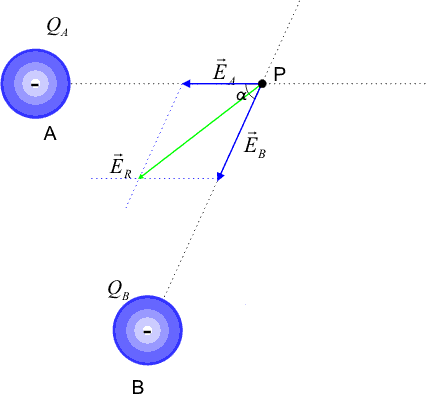
\includegraphics[width=0.37\linewidth]{Figuras/Ch07/varias4.png}}
}

\frame{
	\frametitle{Campo elétrico de várias cargas pontuais fixas}
	\begin{block}{Outro exemplo...}
		Neste exemplo, as cargas que geram o campo resultante têm sinais diferentes, então um dos vetores converge em relação à sua carga geradora ($\vec{E_B}$) e outro diverge ($\vec{E_A}$). \\
		$$\vec{E_R} = \vec{E_A} + \vec{E_B}$$
	\end{block}

	\setmyunit{1.5cm}
	
	\centering
	\begin{tikzpicture}[]
	\draw[dashed] (-1.5,0) -- (2,0) (-60:2) -- (120:0.5);
	
	\draw[-Latex] (0,0) coordinate (O) -- node[above] {$ \vec{E_A} $} (-1,0) coordinate (A);
	\draw[-Latex] (0,0) -- node[right] {$ \vec{E_B} $} (-60:1) coordinate (B);
	
	\draw (A) +(-60:1) coordinate (Ad);
	
	\draw[-Latex,red] (0,0) -- (Ad) node[below,xshift=-7pt] {$ \vec{E_R} $};
	
	\draw[dashed,red] (A) -- (Ad) -- +(-0.5,0) (B) -- (Ad) -- +(-60:0.5);
	
	\fill (0,0) circle (3pt) node[above right=2pt] {$ P $};
	
	\filldraw[fill=white] (2,0) circle (8pt) node[below=8pt] {$ A $} node["$ Q_A $" above] {$ + $};
	
	\filldraw[fill=white] (-60:2) circle (8pt) node[below=8pt] {$ B $} node["$ Q_B $" above] {$ - $};
	
	\pic[ang,gray,->,"$ \alpha $" {xshift=3pt,yshift=-3pt}] {angle=A--O--B};
	\end{tikzpicture}
%	\centerline{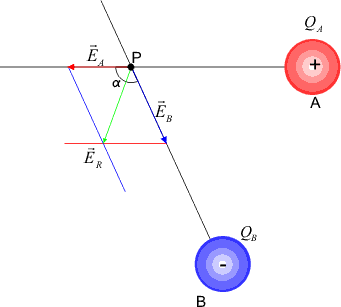
\includegraphics[width=0.4\linewidth]{Figuras/Ch07/varias5.png}}
}

\frame{
	\frametitle{Campo elétrico de várias cargas pontuais fixas}
	\begin{block}{Exemplo \#01}
		Sejam duas cargas $+Q$ e $-Q$ dispostas no vácuo conforme a figura abaixo. Sabe-se que os módulos das cargas são iguais a $Q$. Sendo assim, calcule a intensidade, a direção e o sentido do vetor campo elétrico resultante em $P$. Admita que $Q = \SI{2e-6}{\coulomb}$ e que $ d= $\SI{0.3}{\meter}.
	\end{block}
	
%	\setmyunit{1cm}

	\vspace{0.5cm}
	
	\centering
	\begin{tikzpicture}
	\draw[dashed] (-2,0) -- node[below] {$ d $} (0,0) -- node[below] {$ d $} (2,0);
	
%	\draw[-Latex] (0,0) -- node[above] {$ \vec{E_A} $} (1.5,0);
%	\draw[-Latex] (0,0) -- node[above] {$ \vec{E_B} $} (-1,0);
	
	\fill (0,0) circle (3pt) node[below=2pt] {$ P $};
	
	\filldraw[fill=white] (-2,0) circle (8pt) node["$ +Q $" above] {$ + $} (2,0) circle (8pt) node["$ -Q $" above] {$ - $};
	\end{tikzpicture}
	
%	\centerline{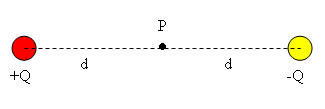
\includegraphics[width=0.4\linewidth]{Figuras/Ch07/varias6.jpg}}
}

\begin{frame}{Campo elétrico de várias cargas pontuais fixas}
	\begin{block}{Resolução}
		Para a carga $+Q$: ela gera em $P$ um $\vec{E_1}$ de afastamento.
		
		Para a carga $-Q$: ela gera em $P$ um $\vec{E_2}$ de aproximação.
		
		$$\vec{E_1} = \vec{E_2} = K \ \dfrac{Q}{d^2} = \num{9e9}\dfrac{ \num{2e-6}}{\num{0,3}^2} =\SI{2e5}{\newton\per\coulomb}$$
		Logo, a intensidade do campo elétrico resultante é $\vec{E} = \vec{E_1} + \vec{E_2} = \num{2e5} + \num{2e5} = \SI{4e5}{\newton\per\coulomb}$. Sua direção é horizontal e o sentido é da esquerda para a direita.
	\end{block}
\end{frame}

\section*{Exercícios}

\frame{
	\frametitle{Exercícios}
	\begin{block}{}

		01. O vetor campo elétrico gerado por uma carga pontual $Q = \SI{8.0}{\micro\coulomb} $, colocada no vácuo, tem intensidade $E = \SI{2.0e5}{\newton\per\coulomb}$, num ponto $P$ situado a uma distância $d$ da carga geradora, na direção horizontal. Determine: 
		
		(a) o valor de $d$.
		
		(b) a intensidade da força que age sobre uma carga de prova $q = \SI{1.0e-7}{\coulomb}$, colocada no ponto $P$.
		
		(c) a direção e sentido da força comparados com o vetor campo elétrico.

		\vspace{0.5cm}

		02. Duas cargas elétricas pontuais $Q_1 = \SI{3.0}{\micro\coulomb}$ e $Q_2 =\SI{5.0}{\micro\coulomb}$ estão situadas a \SI{40}{\centi\meter} uma da outra, sobre uma reta $r$, no vácuo. Determine as características do vetor campo elétrico resultante:
		
		(a) no ponto médio $M$ entre as cargas.
		
		(b) no ponto $P$ situado a \SI{10}{\centi\meter} da carga $Q_1$ sobre a reta $r$, fora da região entre as cargas.
	\end{block}
}


\section*{Referências}

\frame{
	\frametitle{Referências e Exercícios Complementares}
	\begin{itemize}
		\item Física, Ciência e Tecnologia – Vol 3. PENTEADO, Paulo César M; TORRES, Carlos Magno A. Ed. Moderna (2006)
	\end{itemize}
	%\centering{\alert{Página 36 - \textbf{1.6.1 até 1.6.5, 1.6.17 até 1.6.19}}} \\
	%https://www.youtube.com/watch?v=IUgS7Uw-qBI
	\centering{\alert{Lista de exercícios 07}}
}